\documentclass{article}

% Language setting
% Replace `english' with e.g. `spanish' to change the document language
\usepackage[english]{babel}

% Set page size and margins
% Replace `letterpaper' with `a4paper' for UK/EU standard size
\usepackage[a4paper,margin=4cm]{geometry}


% Useful packages
\usepackage{amsmath}
\usepackage{graphicx}
\usepackage[colorlinks=true, allcolors=blue]{hyperref}


\usepackage{geometry}
\geometry{a4paper, margin=1cm, includefoot}
\usepackage{array}
\usepackage[table]{xcolor}
\usepackage{listings}


\usepackage{float}

\usepackage[ruled,vlined]{algorithm2e}


\title{High Performance Computing Project Report}
\author{Simon Wenchel}


\usepackage{appendix}
\usepackage{listings}
\usepackage{xcolor}


\usepackage{amssymb}


\usepackage{todonotes}

\usepackage{hyperref}


\usepackage{booktabs}

\usepackage{subcaption}


\usepackage{cleveref}
% Define code listing style for CPP files
\lstdefinestyle{cppstyle}{
    language=C++,
    basicstyle=\small\ttfamily,
    keywordstyle=\color{blue},
    commentstyle=\color{green!60!black},
    stringstyle=\color{red},
    numbers=left,
    numberstyle=\tiny,
    numbersep=5pt,
    breaklines=true,
    showstringspaces=false,
    frame=tb,
    captionpos=b,
    tabsize=4
}

\begin{document}
\maketitle

\begin{abstract}
In this report the work on my HPC-project will be explained and the results will be shown.

\end{abstract}

\section{Assignment}
Consider the transient convection-diffusion equation in $1\mathrm{D}$:

$$
-D \frac{\partial^{2} c}{\partial x^{2}}-v_{x} \frac{\partial c}{\partial x}=\frac{\partial c}{\partial t} \quad 0 \leq x \leq L, \quad t \geq 0
$$

with boundary conditions:

$$
\left\{\begin{array}{l}
c(0, x)=\bar{c} \\
\left.D \frac{\partial c}{\partial x}\right|_{x=L}=\bar{q}
\end{array}\right.
$$
\\
Discetization leads to the algebraic system:
$$
(H+B)c+P\frac{\mathrm{d}c}{\mathrm{d}t} - q = 0 \text{ ,}
$$
where $H$,$B$,$P$ are tridiagonal matrices.\\\\
In the $2 \mathrm{D}$ case the convection-diffusion equation becomes:

$$
\frac{\partial}{\partial x}\left(D_{x} \frac{\partial c}{\partial x}\right)+\frac{\partial}{\partial y}\left(D_{y} \frac{\partial c}{\partial y}\right)-v_{x} \frac{\partial c}{\partial x}-v_{y} \frac{\partial c}{\partial y}=\frac{\partial c}{\partial t} \quad+f
$$

with boundary conditions:

$$
\left\{\begin{array}{l}
c(x, y, t)=\bar{c},(t) \quad \forall(x, y) \in \partial \Omega_{1} \\
D_{x} \frac{\partial u}{\partial x} n_{x}+D_{y} \frac{\partial u}{\partial y} n_{y}=\bar{q}, \quad \forall(x, y) \in \partial \Omega_{2}
\end{array}\right.
$$
\\
The local contributions of the element $e$ on the entries $h_{i j}$ of the stiffness matrix $H$ and $p_{i j}$ of the capacity matrix $P$ read:

$$
\begin{aligned}
h_{i j}^{(e)} & =\int_{\Delta_{e}}\left(D_{x} \frac{\partial \xi_{i}^{(e)}}{\partial x} \frac{\partial \xi_{j}^{(e)}}{\partial x}+D_{y} \frac{\partial \xi_{i}^{(e)}}{\partial y} \frac{\partial \xi_{j}^{(e)}}{\partial y}\right) \mathrm{d} x \mathrm{~d} y=\frac{D_{x} b_{i} b_{j}+D_{y} c_{i} c_{j}}{4 \Delta_{e}} \\
p_{i j}^{(e)} & =\int_{\Delta_{e}} \xi_{i}^{(e)} \xi_{j}^{(e)} \mathrm{d} x \mathrm{~d} y= \begin{cases}\Delta_{e} / 6 & i=j \\
\Delta_{e} / 12 & i \neq j\end{cases}
\end{aligned}
$$

where $b_{i}, b_{j}, c_{i}$ e $c_{j}$ are computed using the triangle $e$ coordinates. If $i$ is a node belonging to the Neumman boundary $\partial \Omega_{2}$, the contribution to the $i$-th right-hand side component arises from (4):

$$
q_{i}^{(e)}=\int_{\partial \Omega_{2}^{(e)}} \bar{q} \xi_{i}^{(e)} \mathrm{d} S=\bar{q} \frac{l^{(e)}}{2}
$$

with $l^{(e)}$ the length of the side a triangle belonging to $\partial \Omega_{2}$ and the node $i$ as vertex.

The $b_{i j}$ entry of the convective matrix $B$ is given by:
$$
b_{i j}=\int_{\Omega}\left(v_{x} \frac{\partial \xi_{j}}{\partial x}+v_{y} \frac{\partial \xi_{j}}{\partial y}\right) \xi_{i} \mathrm{~d} x \mathrm{~d} y
$$



\newpage

To solve this problem two main tasks need to be handled:
\begin{enumerate}
    \item The assembly of the linear system given a predefined mesh structure.
    \item The efficient solution of the large linear system obtained
\end{enumerate}
The primary objective of this report is to highlight the implementation of parallel programming paradigms as the preferred solution for these tasks.


\section{Implementation Framework}
\subsection{Used OpenMP Paradigms}
OpenMP is a programming model that helps in parallelizing tasks on shared memory architectures by dividing the work into smaller tasks that can be executed concurrently by multiple threads.\\
The number of threads can be set in the terminal with command:
\begin{verbatim}
export OMP_NUM_THREADS=n
\end{verbatim}

\subsubsection{\texttt{for}}
The \texttt{for} paradigm is used to parallelize loops. It divides the iteration between the available threads. 
\begin{verbatim}
#pragma omp parallel for
for (int i = 0; i < n; i++) {
    // do something
    // ...
}
\end{verbatim}

\subsubsection{\texttt{schedule}}
The \texttt{schedule} command is used with \texttt{for} loops to decide how threads are scheduled.
In this project, we use the \texttt{dynamic} scheduling approach as shown in the following example.
Using dynamic scheduling helps reduce the amount of time threads spend waiting.
The formula \texttt{n/1000+1} determines the size of each chunk.
After a thread finishes processing one chunk, it receives a smaller chunk to prevent a situation where all threads have to wait for one thread to finish.
\begin{verbatim}
#pragma omp parallel for schedule(dynamic, n/1000+1)
for (int i = 0; i < n; i++) {
    // do something
    // ...
}
\end{verbatim}

\subsubsection{\texttt{reduction}}
\texttt{reduction} is used for reducing a simple operation, such as summation or multiplication, on a variable over multiple threads. Pairwise operations will be done such that the number of total operations is reduced by half each step.
\begin{verbatim}
int sum = 0;
#pragma omp parallel for reduction(+:sum)
for (int i = 0; i < n; i++) {
    sum += array[i];
}
\end{verbatim}

\subsubsection{\texttt{atomic}}
\texttt{atomic} ensures that a special location in the memory is only accessed by one thread at a time to prevent data race. This leads to potential performance reduction as the threads may need to wait to access the desired memory location.
\begin{verbatim}
#pragma omp parallel for
for (int i = 0; i < n; i++) {
    #pragma omp atomic
    counter++;
}
\end{verbatim}

\subsubsection{\texttt{critical}}
The clause \texttt{critical} makes sure that only one thread enters a special section in the code. This also reduces performance because threads may need to wait for executing the \texttt{critical} code.
\begin{verbatim}
#pragma omp parallel for
for (int i = 0; i < 10; i++) {
        // do something
        // ..
        #pragma omp critical
        {
            // do something only one thread is allowed once at a time
        }
    }
\end{verbatim}

\subsection{Data Structures and Basic Functions}
\subsubsection{The Compressed Sparse Row Format (CSR)}
The CSR format is widely used representation to store large sparse matrices in an efficient way and minimize the needed memory.\\
In the project, we only deal with square matrices. That's why, for the explanations, we only consider square matrices and look at an $n \times n$ matrix with $n_{\text{term}}$ entries.\\
The standard approach in storing a sparse matrix would be storing three lists containing the column and row index and the value of the non-zero elements. This leads to a memory occupation of $\mathtt{n\_{term}}  (2\cdot\mathtt{sizeof(int)} + \mathtt{sizeof(double)})$\\
As shown in Table \ref{tab:CSR} the CSR format also has three lists but needs $\mathtt{n\_term} - \mathtt{n}$ fewer elements. The larger the matrix and the more non-zero elements the matrix get this format gets more efficient. 
\begin{table}[h]
\centering
\renewcommand{\arraystretch}{1.5}
\begin{tabular}{|p{3cm}|p{2cm}|p{2cm}|p{9cm}|}
\hline
\rowcolor{gray!20}
\textbf{Name} & \textbf{Data Type} & \textbf{Length} & \textbf{Explanation} \\
\hline
\lstinline|values| & \lstinline|double*| & \lstinline|n_term| & Array storing the non-zero values of the matrix \\
\hline
\lstinline|column_indices| & \lstinline|int*| & \lstinline|n_term| & Array storing the column indices of the corresponding non-zero values \\
\hline
\lstinline|row_pointers| & \lstinline|int*| & \lstinline|nrow + 1| & Array storing the indices where each row starts in the \lstinline|values| and \lstinline|column_indices| arrays last index for these arrays\\
\hline
\end{tabular}
\caption{Arrays for CSR Format}
\label{tab:CSR}
\end{table}

\subsubsection{The Sparse Class}
The CSR format was utilized for creating an own data structure to store and manage large sparse matrices in the code all attributes and methods of this class are shown in Table \ref{tab:UML}. In the following special functions and their parallelization will be explained.

\begin{table}[h]
\centering
\renewcommand{\arraystretch}{1.5}
\begin{tabular}{|p{8cm}|p{3cm}|p{7cm}|}
\hline
\rowcolor{gray!20}
\textbf{Class Name} & \multicolumn{2}{p{11cm}|}{sparse} \\
\hline
\multicolumn{3}{|p{16cm}|}{\textbf{Private Members}} \\
\hline
\lstinline|nrow| & \lstinline|int| & Number of rows \\
\hline
\lstinline|ncol| & \lstinline|int| & Number of columns \\
\hline
\lstinline|n_term| & \lstinline|int| & Number of non-zero matrix elements \\
\hline
\lstinline|coef| & \lstinline|double*| & Pointer to non-zero matrix elements \\
\hline
\lstinline|iat| & \lstinline|int*| & Pointer to the first non-zero column index \\
\hline
\lstinline|ja| & \lstinline|int*| & Pointer to the column indices \\
\hline
\multicolumn{3}{|p{16cm}|}{\textbf{Public Members}} \\
\hline
\lstinline|sparse()| & sparse & Default constructor \\
\hline
\lstinline|sparse(int nrow, int ncol, int n_term)| & sparse & Parameterized constructor \\
\hline
\lstinline|~sparse()| & void & Destructor \\
\hline
\multicolumn{3}{|p{16cm}|}{\textit{Get and Set Methods}} \\
\hline
\lstinline|full2sparse(double** A, int n_row)| & void & Convert full matrix to sparse \\
\hline
\lstinline|addition_update(sparse* B_ptr)| & void & Addition and update operation \\
\hline
\lstinline|scalarMult(double alpha)| & void & Scalar multiplication \\
\hline
\lstinline|post_MV(double* v, double* y)| & void & Matrix-vector multiplication \\
\hline
\lstinline|pre_MV(double* v, double* y)| & void & Vector-matrix multiplication \\
\hline
\lstinline|matrixProduct(sparse* A_ptr, sparse* result)| & void & Matrix product \\
\hline
\lstinline|diag(double* v)| & void & diagonal submatrix $D$ \\
\hline
\lstinline|getJacobi(double* v)| & void & Inverse of the Diagonal matrix $D^{-1}$\\
\hline
\lstinline|diag_x_sparse(double* diag)| & void & Diagonal matrix times sparse \\
\hline
\lstinline|left_Jacobi()| & double* & Left Jacobi preconditioning $D^{-1}A$ \\
\hline
\lstinline|printMat()| & void & Print matrix \\
\hline
\lstinline|printComponents()| & void & Print components \\
\hline
\end{tabular}
\caption{UML Diagram of the \texttt{sparse} Class}
\label{tab:UML}

\end{table}


\paragraph{Matrix-vector Product \lstinline|postMV|} computes the matrix-vector product $Av=y$ in a parallel and efficient way.\\\\
\begin{minipage}[t]{0.45\textwidth}
Explanation:
\begin{itemize}
    \item outer loop iterates over each row as each row gets multiplied with the vector
    \item inner loop iterates from the first element in the row \lstinline|i| \lstinline |iat[i]| to the last element in the row \lstinline |iat[i]|-1
    \item This is embarrassingly parallel as the rows have no relation as well as the saved component for each \lstinline|y|
\end{itemize}
\end{minipage}
\hspace{0.7cm}
\begin{minipage}[t]{0.35\textwidth}
Code:
\begin{verbatim}
void post_MV(double* v, double* y ){
    #pragma omp parallel for \\
            schedule(dynamic,nrow/1000+1)
    for(int i=0; i<nrow; i++){
        double sum = 0.0;
        // #pragma omp simd reduction(+:sum)
        for(int j=iat[i]; j<iat[i+1]; j++){
            sum += coef[j]*v[ja[j]];
        }
        y[i] = sum;
    }
}


\end{verbatim}
\end{minipage}

\paragraph{Jacobi Preconditioning}
Computes the Matrix multiplied by the Jacobi preconditioner from the left side. The left side multiplication utilizes the CSR format because it is easier to iterate over each row. This is done by four methods.\\\\

% \begin{enumerate}
%     \item \lstinline|getJacobi|
%     \item  \lstinline|diag_x_sparse|
%     \item  \lstinline|leftJacobi|
% \end{enumerate}
% \hspace{.01cm}
\begin{minipage}[t]{0.45\textwidth}
Explanation:
\begin{itemize}
    \item the diagonal matrix is represented as an 1-D array, of which all values were set to zero before function call 
    \item loops are the same as in matrix-vector product
    \item stop iterating in the row when diagonal index is met
    \item also embarrassingly parallel as the rows have no relation as well as the saved component for each \lstinline|v|
\end{itemize}
\end{minipage}
\hspace{0.7cm}
\begin{minipage}[t]{0.35\textwidth}
Code:
\begin{verbatim}
void diag(double* v) {
    int start, end;
    #pragma omp parallel for \\
            schedule(dynamic, ncol/1000 + 1)
    for(int i = 0; i < ncol; i++) {
        start = iat[i];
        end = iat[i + 1];
        for(int j = start; j < end; j++) {
            if (ja[j] == i) {
                v[i] = coef[j];
                break;
            }
        }
    }
}


\end{verbatim}
\end{minipage}

\begin{minipage}[t]{0.45\textwidth}
\begin{itemize}
    \item compute inverse of diagonal matrix $D$
    \item prevent division by zero and set diagonal element to one s.t. no change in that row will take place
    \item count the zeros as the effectiveness of Jacobi reduces with increasing number of zeroes
\end{itemize}
\end{minipage}
\hspace{0.7cm}
\begin{minipage}[t]{0.35\textwidth}
\begin{verbatim}
void getJacobi(double* v) {
    this->diag(v);
    int zeros = 0;
    #pragma omp parallel for \\
            schedule(dynamic, ncol/1000 + 1)
    for(int i = 0; i < ncol; i++) {
        if (v[i] == 0) {
            v[i] = 1;
            #pragma omp atomic
            zeros++;
        }
        v[i] = 1 / v[i];
    }
    if (zeros > 0) {
        cout << "WARNING: Number of zeros\\
        in diagonal: " << zeros << endl;
    }
}


\end{verbatim}
\end{minipage}

\begin{minipage}[t]{0.45\textwidth}
\begin{itemize}
    \item loops are the same as in Matrix-vector product
    \item simplified matrix product because of diagonal structure
    \item every element in row \lstinline|i| is multiplied by \lstinline|v[i]|
\end{itemize}
\end{minipage}
\hspace{0.7cm}
\begin{minipage}[t]{0.35\textwidth}
\begin{verbatim}
void diag_x_sparse(double* diag) {
    int start, end;
    #pragma omp parallel for \\
            schedule(dynamic, ncol/1000 + 1)
    for(int i = 0; i < ncol; i++) {
        start = iat[i];
        end = iat[i + 1];
        for(int j = start; j < end; j++) {
            coef[j] *= diag[i]; 
        }
    }
}


\end{verbatim}
\end{minipage}




\begin{minipage}[t]{0.45\textwidth}
\begin{itemize}
    \item allocate array with guaranteed zeroes in every entry
    \item compute the preconditioned matrix
\end{itemize}
\end{minipage}
\hspace{0.7cm}
\begin{minipage}[t]{0.35\textwidth}
\begin{verbatim}
double* left_Jacobi() {
    double* v =(double*)calloc(ncol,sizeof(double));
    this->getJacobi(v);
    this->diag_x_sparse(v);
    return v;
}


\end{verbatim}
\end{minipage}




\subsubsection{Basic Linear Algebra Operations}
In the following basic functions for standard operations are described. Some others are equivalent and can be found in the complete code.
\paragraph{Scalar Product} calculate the standard scalar product of two vectors.\\\\
\begin{minipage}[t]{0.45\textwidth}
Explanation:
\begin{itemize}
    \item perfect use for the reduction clause
    \item reduction does not need an atomic statement
    \item embarrassingly parallel
\end{itemize}
\end{minipage}
\hspace{.7cm}
\begin{minipage}[t]{0.35\textwidth}
Code:
\begin{verbatim}
double scalar_prod(double *v1, double *v2, int nr){
    double sum = 0.0;
    #pragma omp parallel for reduction(+:sum)
    for(int i = 0; i < nr; i++){
        sum += v1[i] * v2[i];
    }
    
    return sum;
}
\end{verbatim}
\end{minipage}

\paragraph{Vector Update}
Add a vector onto another and scale it with a factor.\\\\
\begin{minipage}[t]{0.45\textwidth}
Explanation:
\begin{itemize}
    \item standard parallel for loop
    \item embarrassingly parallel
\end{itemize}
\end{minipage}
\hspace{.7cm}
\begin{minipage}[t]{0.35\textwidth}
Code:
\begin{verbatim}
void vector_update(double *v1, double *p,\\
                    double alpha, int nr) {
    #pragma omp parallel for \\
            schedule(dynamic, nr/1000+1)
    for (int i = 0; i < nr; ++i) {
        v1[i] += alpha * p[i];
    }
}

\end{verbatim}
\end{minipage}

\paragraph{Upper Triangular System Solver}
Solving an upper triangular system using backward substitution is straightforward. However, when working with large systems, efficient parallelization row-by-row is difficult due to the dependency on solving the rows below first. The basic operation is $$\mathtt{x[row]} = 
\big(\mathtt{b[row]}-\sum_{\mathtt{col} = \mathtt{row}+1}^{n} \mathtt{A[row][col]} \cdot \mathtt{x[col]}\big)/\mathtt{A[row][row]}$$
To parallelize this process, the reduction operator can be used as the summation grows with each iteration of \lstinline|row|. However, it needs to be evaluated if the size of the system being solved is large enough to actually improve the performance using parallelization. \\\\
Code:
\begin{verbatim}
void triangularSolver(double** A, double* b,\\
                        double* x, int n) {
    for (int row = n - 1; row >= 0; row--) {
        double sum = 0.0;
        #pragma omp parallel for reduction(+:sum)
        for (int col = row + 1; col < n; col++) {
            sum += A[row][col] * x[col];
        }
        x[row] = (b[row] - sum) / A[row][row];
    }
}


\end{verbatim}
\paragraph{Maximum}
Finding the maximum value in an array utilizing parallelization can be achieved by using the \lstinline|critical| directive to prevent data races. This is necessary because other threads may have modified the \lstinline|maxVal| variable in the meantime. The code snippet provided demonstrates the usage of \lstinline|critical| to ensure that the comparison \lstinline|v[i] > maxVal| is still valid before updating \lstinline|maxVal| if needed.
\begin{verbatim}
double max(double* v, int n) {
    double maxVal = v[0];
    #pragma omp parallel for \\
            schedule(dynamic, n/1000+1)
    for (int i = 1; i < n; i++) {
        if (v[i] > maxVal) {
            #pragma omp critical
            {
                if (v[i] > maxVal) {
                    maxVal = v[i];
                }
            }
        }
    }
    return maxVal;
}



\end{verbatim}
\section{Assembly}
\subsection{Mesh Data}
For the solution we used a non overlapping triangulation of $\Omega$ with triangular finite elements. The input data is shown in Table \ref{tab:meshinput}.
\begin{table}[htbp]
    \centering
    \begin{tabular}{l|l|c}
        \toprule
        \rowcolor{gray!20}
        \textbf{File Name} & \textbf{File containing} & \textbf{Input Representation} \\
        \midrule
        \texttt{mesh} & number of elements \texttt{ne} & 800\\
         &the triangle topology & \text{ }\texttt{1       23      22} \\
         & & \texttt{22      44      43} \\
         & & \texttt{43      65      64} \\
         & &  $\ldots$ $\ldots$ \\
         & & \\
        \texttt{coord} & number of nodes \texttt{nn} & 441\\
         & the node coordinates & \texttt{0.0 1.00} \\
         & & \texttt{0.0 0.95} \\
         & & \texttt{0.0 0.90} \\
         & & $\ldots$  $\ldots$ \\
         & & \\
        \texttt{bound} & number of dirichlet nodes \texttt{nb} & 80\\
         & the set of Dirichlet nodes and their values & \texttt{1 1.0} \\
         & & \texttt{2 1.0} \\
         & & \texttt{3 1.0} \\
         & & $\ldots$ \\
         & & \\
        \bottomrule
    \end{tabular}
    \caption{Description of the input files describing the mesh.}
    \label{tab:meshinput}
\end{table}
\subsection{Nonzero Structure of the System Matrix}
Determining the nonzero structure of a matrix is essential before further computations can proceed, especially in the CSR format. Changing a zero to a nonzero value is not feasible without storing a new matrix. A matrix entry, denoted as $H_{i,j}$, is considered nonzero if and only if two finite elements share nodes $i$ and $j$.\\
The mesh topology input allows for an easy derivation of this pattern. We construct the adjacency matrix $A$ with \texttt{nn} rows and \texttt{ne} columns, where each element will have a 1 at every node that is part of it. \\ 
The final pattern of the system matrix is then received by the product: $H = A^TA$.This is shown in the code below. \\
\begin{verbatim}
void stiffness_struct(char* fname, int ne, int nn, double** topol) {
    double** Adj = mat_allocation(ne, nn);
    double* i_idx = (double*)malloc(static_cast<int>(nn * nn * 0.2));
    double* j_idx = (double*)malloc(static_cast<int>(nn * nn * 0.2));

    int idx;
    #pragma omp parallel for schedule(dynamic, nn / 1000 + 1)
    for (int i = 0; i < ne; i++) {
        for (int k = 0; k < 3; k++) {
            idx = static_cast<int>(floor(topol[i][k]) - 1);
            Adj[i][idx] = 1;
        }
    }

    double sum;
    int nnz = 0;
    std::string tempFile = "temp_file.txt";
    std::ofstream file(tempFile, std::ofstream::trunc); // Open the temporary file in write mode with truncation
    for (int i = 0; i < nn; i++) {
        for (int j = 0; j < nn; j++) {
            sum = 0;
            for (int k = 0; k < ne; k++) {
                sum += Adj[k][i] * Adj[k][j];
            }
            if (sum > 0) {
                nnz++;
                file << j + 1 << " " << i + 1 << " " << 0 << std::endl;
            }
        }
    }
    file.close();
}


\end{verbatim}

This technique works perfectly fine for small meshes, but with growing meshsize the performance and memory consumption are the reason why this is not working.\\
Therefore another function with way less memory consumption and operations was implemented as shown below.\\
In this version the creation of the adjacency matrix is omitted and the indices are saved directly to be ordered afterwards and than added to the CSR matrix structure directly. This could be parallelized with only adjusting vector containers by using the \texttt{atomic} operator or creating subvectors and merging them after the loop, it would be solved.\\
This approach lead to unsolvable errors and was not continued because of time consumption.
\begin{verbatim}
	void stiffness_struct_small_loops(sparse* H, int ne, int nn, double** topol) {
    // Create vectors to store the i_idx and j_idx pairs
    std::vector<int> i_idx;
    std::vector<int> j_idx;
    
    // Loop through each element
    for (int i = 0; i < ne; i++) {
        for (int k = 0; k < 3; k++) {
            int idx = static_cast<int>(floor(topol[i][k]) - 1);
            for (int l = 0; l < 3; l++) {
                int jdx = static_cast<int>(floor(topol[i][l]) - 1);
                i_idx.push_back(idx);
                j_idx.push_back(jdx);
            }
        }
    }
    
    // Combine i_idx and j_idx into pairs for sorting
    std::vector<std::pair<int, int>> pairs;
    for (int i = 0; i < i_idx.size(); i++) {
        pairs.push_back(std::make_pair(i_idx[i], j_idx[i]));
    }
    
    // Sort the pairs to bring duplicates together
    std::sort(pairs.begin(), pairs.end());
    
    // Remove duplicates and copy the unique pairs back to i_idx and j_idx
    int nnz = 0;
    for (int i = 0; i < pairs.size(); i++) {
        if (i == 0 || pairs[i] != pairs[i - 1]) {
            i_idx[nnz] = pairs[i].first + 1;
            j_idx[nnz] = pairs[i].second;
            nnz++;
        }
    }
    
    // Allocate memory for the CSR arrays
    int* ja_loc = new int[nnz];
    int* iat_loc = new int[nn + 1];
    
    // Copy the data from i_idx and j_idx to the CSR arrays
    for (int i = 0; i < nnz; i++) {
        ja_loc[i] = j_idx[i];
    }
    
    // Compute the CSR arrays from i_idx and ja_loc
    irow2iat(nn, nnz, &i_idx[0], iat_loc);
    
    H->set_n_term(nnz);
    H->set_ncol(nn);
    H->copy_ja(ja_loc);
    H->copy_iat(iat_loc);

    delete[] ja_loc;
    delete[] iat_loc;
}

	
\end{verbatim}
 %Because of time reasons debugging was stopped 
\subsection{Computation of the Right Hand Side}
The right hand side is composed of the forcing function $f$ and the boundary condition that is also given as input file. In this report the forcing function is zero always.
\subsection{Boundary Condition Enforcement}
The boundary condition is enforced with the penalty method with the value $10^{15}$
\begin{verbatim}
void imposeBC(sparse* H, double** bound, double* q, int nb){
	double R = 1e15;
	int j, bound_idx, start, end;
	int* iat = H->get_iat();
	int* ja = H->get_ja();
	double* coef = H->get_coef();
	
	for(int i = 0; i<nb; ++i){
		bound_idx = static_cast<int>(bound[i][0])-1;
		start = iat[bound_idx];
		end = iat[bound_idx+1];
		
		for(j = start; j<end; j++){
			if (ja[j] == bound_idx){break;}
		}
		
		coef[j] = R;
		q[bound_idx] = R*bound[i][1];
	}
}
\end{verbatim}
\section{Generalized Minimal Residual Algorithm}
GMRES is an iterative method to solve linear systems of equations. The solution is approximated by the Krylov subspace with minimal residual.
\subsection{The Householder Version}
The orthogonalization in the Arnoldi process is commonly performed using the Gram-Schmidt procedure, which can suffer from numerical instability. However, an alternative technique known as Householder projections provides improved numerical stability for the orthogonalization step. The Householder projection matrix is defined as $P = I - 2u^Tu$, where $u$ is a unit vector. This definition can be utilized in the GMRES algorithm as only the vector $v$ needs to be stored to define a $P_i$ as well as $P_iv = v-u^Tuv$ where the matrix-vector product reduces to simple vector operations.\\
In Algorithm \ref{alg:gmres} GMRES with Householder projections is presented taken from \cite{saad}, who developed this method in 1986.\\
\begin{algorithm}[h]
\LinesNumbered
\SetAlgoLined
\SetKwInOut{Input}{Input}
\SetKwInOut{Output}{Output}

\Input{$A$, $b$, $m$, $x_0$}
\Output{$x_m$}

Compute $r_0 = b - Ax_0$, $z = r_0$\;
\For{$j = 1, \ldots, m, m+1$}{
    Compute the Householder unit vector $w_j$ such that\\
    $w_j(i) = 0, i = 1, \ldots, j-1$ and $(P_jz)(i) = 0, i = j+1,\ldots, n$\\
    where $P_j = I - 2w_jw_j^T$\;
    $h_{j-1} = P_jz$\;
    \If{$j = 1$}{
        Let $\beta = e^T_1h_0$\;
    }
    $v = P_1P_2 \ldots P_jw_j$\;
    \If{$j \leq m$}{
        Compute $z = P_jP_{j-1} \ldots P_1Av$\;
    }
}
Define $\bar{H}_m$ as the $(m+1) \times m$ upper part of the matrix $[h_1, \ldots, h_m]$\;
Compute $y_m = \text{Argmin}_y \lVert \beta e_1 - \bar{H}_my \rVert_2$\;
Let $y_m = (\eta_1, \eta_2, \ldots, \eta_m)^T$\;
$z = 0$\;
\For{$j = m, m-1, \ldots, 1$}{
    $z = P_j(\eta_j e_j + z)$\;
}
Compute $x_m = x_0 + z$\;

\caption{GMRES Algorithm with Householder projections}\label{alg:gmres}
\end{algorithm}
\paragraph{Givens Rotation}
Saad also suggests in his book to use Givens rotations to transform the linear system, that needs to be solved in line 16, from Householder structure to an upper triangular matrix making it easy to solve.\\
The rotation matrix $\Omega_i$ is defined as \\
\begin{minipage}{0.5\textwidth}
    \[
    \Omega_i=\left(\begin{array}{cccccccc}
    1 & & & & & & & \\
    & \ddots & & & & & & \\
    & & 1 & & & & & \\
    & & & c_i & s_i & & & \\
    & & & -s_i & c_i & & & \\
    & & & & & 1 & & \\
    &  & & & & &\ddots & \\
    & & & & & & & 1
    \end{array}\right)
    \]
\end{minipage}%
\begin{minipage}{0.5\textwidth}
    with \(c_i^2+s_i^2=1\) and \(c_i\) and \(s_i\) of the \(i^{\text{th}}\) rotation
    \[
    s_i=\frac{h_{i+1, i}}{\sqrt{\left(h_{i i}^{(i-1)}\right)^2+h_{i+1, i}^2}}, \quad c_i=\frac{h_{i i}^{(i-1)}}{\sqrt{\left(h_{i i}^{(i-1)}\right)^2+h_{i+1, i}^2}} .
    \]
\end{minipage}

Applying the rotation matrices on $\bar{H}_4$ the transformed system is shown below.
$$
\bar{H}_4=\left(\begin{array}{lllll}
h_{11} & h_{12} & h_{13} & h_{14}  \\
h_{21} & h_{22} & h_{23} & h_{24} \\
& h_{32} & h_{33} & h_{34}  \\
& & h_{43} & h_{44}  \\
& & & h_{54}  \\
\end{array}\right), \quad \bar{g}_0=\left(\begin{array}{c}
\beta \\
0 \\
0 \\
0 \\
0 \\

\end{array}\right) .
$$
$$
\bar{H}_4^{(4)}=\left(\begin{array}{ccccc}
h_{11}^{(4)} & h_{12}^{(4)} & h_{13}^{(4)} & h_{14}^{(4)} \\
& h_{22}^{(4)} & h_{23}^{(4)} & h_{24}^{(4)} \\
& & h_{33}^{(4)} & h_{34}^{(4)}  \\
& & & h_{44}^{(4)}  \\
& & & 0
\end{array}\right), \quad \bar{g}_4=\left(\begin{array}{c}
\gamma_1 \\
\gamma_2 \\
\gamma_3 \\
\gamma_4 \\
\gamma_5 \\

\end{array}\right)
$$

\paragraph{Restarting}
Another suggestion from Saad is to apply restarting after some iterations to the GMRES algorithm. This is beneficial since the start vector improves by every restart and so does the generated Krylov subspace. Another improvement is that the triangular system to solve is relatively small as well as the matrices that store projections or the transformed Hessenberg matrix. For the standard GMRES the convergence is guaranteed after $n$ iterations. This property gets lost with the restarted version, but since $n$ is large this property is impractical.\\
The algorithm \ref{alg:gmres-restarted} is also taken from \cite{saad}.\\
\begin{algorithm}[h]
\LinesNumbered
\SetAlgoLined
\SetKwInOut{Input}{Input}
\SetKwInOut{Output}{Output}

\Input{$A$, $b$, $m$, $x_0$}
\Output{$x_m$}

Compute $r_0 = b - Ax_0$, $\beta = \lVert r_0 \rVert_2$, and $v_1 = r_0 / \beta$\;
Generate the Arnoldi basis and the matrix $\bar{H}_m$ using the Arnoldi algorithm starting with $v_1$\;
Compute $y_m$ which minimizes $\lVert \beta e_1 - \bar{H}_m y \rVert_2$\;
If satisfied, then Stop. Otherwise, set $x_0 := x_m$ and go to Step 1\;

\caption{Restarted GMRES}\label{alg:gmres-restarted}
\end{algorithm}

\subsection{Implementation}
In the following, parts of the implemented GMRES will be written down in pseudo-code and details of the implementation will be explained. When an operation is parallelized, it is mentioned once. Subsequent occurrences of the same operation are parallelized as well, without explicitly mentioning.\\
The restarted part will be omitted in this explanation since it is straightforward.\\
The full GMRES implementation can be viewed in the appendix Code \ref{code:GMRES}.\\
The input values can be viewed in table \ref{tab:gmres-input}. The function does not have a return value the solution vector is stored in start vector from the input. \\


\begin{table}[h]
\centering
\renewcommand{\arraystretch}{1.5}
\begin{tabular}{|p{3cm}|p{3cm}|p{10cm}|}
\hline
\rowcolor{gray!20}
\textbf{Name} & \textbf{Data Type} & \textbf{Explanation} \\
\hline
\lstinline|z_ptr| & \lstinline|sparse*| & Pointer to the sparse matrix of the linear system to be solved \\
\hline
\lstinline|b| & \lstinline|double*| & Pointer to the right-hand side array \\
\hline
\lstinline|x| & \lstinline|double*| & Pointer to the start and solution array \\
\hline
\lstinline|preconditioning| & \lstinline|bool| & Boolean indicating whether preconditioning is used \\
\hline
\lstinline|restarting| & \lstinline|bool| & Boolean indicating whether restarting is used \\
\hline
\lstinline|maxit| & \lstinline|int| & Maximum number of iterations \\
\hline
\end{tabular}

\caption{Input variables for the GMRES function.}
\label{tab:gmres-input}
\end{table}

\paragraph{Arnoldi process}
In Algorithm \ref{alg:gmres-househ} the Arnoldi process with Householder projections of my implementation is presented and parts of the parallelization are mentioned. The parallelization can just be applied on single operations as there is data dependence on the outer loops or even the application of the projection matrices.\\
\begin{algorithm}[h]
\LinesNumbered
\SetAlgoLined
\SetKwInOut{Input}{Input}
\SetKwInOut{Output}{Output}

\Input{$A$, $x$, $b$, $U\in \mathbb{R}^{n \times inner}$}
\Output{$x_m$}

Compute $r = b - Ax$, $u = r$, $normr = ||r||$, $\beta = \text{sig}(normr)\cdot normr$, $u = r$ \\
$\qquad \qquad$$u_0 = u_0 + \beta$, $u = \frac{u}{||u||}$, $U_{0,:} = u$, $w_0 = - \beta$ \;
\For{$j = 1, \ldots, outer$}{
\For{$i = 1, \ldots, inner$}{
    $v = -2u_{i}\cdot u^{(i)}$ ; \tcp*[h]{scalar multiplication done in parallel}\\
    $v_{i} += 1$; \tcp*[h]{just update one value}\\
    \tcp*[h]{do: $v = P_1\cdots P_{i} e_{i}$, but why ei?} \\
    \For{$k = i-1 \ldots 0$}{
        $v = v - 2 {u^{(k)}}^Tu^{(k)}\cdot v$; \tcp*[h]{scalar product and vector update is parallelized}\\
    }
    $v = \frac{v}{||v||}$; \tcp*[h]{normalization is parallel} \\

    \tcp*[h]{do: $v = P_i\cdots P_{0} Av$} \\
    $v = Av$; \tcp*[h]{sparse Matrix-vector product is parallel}\\
    \For{$k = 0 \ldots i$}{
        $v = v - 2 {u^{(k)}}^Tu^{(k)}\cdot v$;\\
    }    
    \tcp*[h]{compute $u^{i+1}$ for $P_{j+1}$}\\
    $u^{i+1} = v$\;
    $u_{0:initer} = 0$; \tcp*[h]{zero\_out is parallel}\\
    $\alpha = ||u||$; \tcp*[h]{norm is parallel}\\
    \If{$alpha>0$}{
        $\alpha = v_{i+1}\alpha$\;
        $u^{(i+1)}_{i+1} = u^{(i+1)}_{i+1}+\alpha$\;
        \tcp*[h]{normalize $u^{(i+1)}$}\;
        \tcp*[h]{do $v = P_{i+1}v$} \\
        $v_{i+1:n} = 0$\;
        $v_{i+1} = -\alpha$\;
    }

    \tcp*[h]{Continue with Givens rotation...} \\
    \tcp*[h]{...}\\
}
}
\caption{Householder part}\label{alg:gmres-househ}
\end{algorithm}
\paragraph{Givens Rotation}
In Algorithm \ref{alg:gmres-givens} the givens rotation to obtain the triangular system is explained. In this part no real parralelization can be done because the operations are mostly on scalars and not Vectors that can be divided in parallel calculations.\\
\begin{algorithm}[h]
\LinesNumbered
\SetAlgoLined


\For{$j = 1, \ldots, \text{outer}$}{
\For{$i = 1, \ldots, \text{inner}$}{
    \tcp*[h]{...}\\
    \tcp*[h]{Previous code...}\\
    \tcp*[h]{Continue with Givens rotation...} \\
    $j_0 = v_i$; \tcp*[h]{Store $v_i$ in $j_0$} \\
    $j_1 = v_{i+1}$; \tcp*[h]{Store $v_{i+1}$ in $j_1$} \\
    $\rho = \sqrt{j_0^2 + j_1^2}$; \tcp*[h]{Compute the norm} \\
    $j_0 = \frac{j_0}{\rho}$; \tcp*[h]{Normalize $j_0$} \\
    $j_1 = \frac{j_1}{\rho}$; \tcp*[h]{Normalize $j_1$} \\
    $J_{i,0} = j_0$; \tcp*[h]{Store the Givens rotation values} \\
    $J_{i,1} = j_1$; \tcp*[h]{Store the Givens rotation values} \\
    $w_{i+1} = -J_{i,1} \cdot w_i$; \tcp*[h]{Update $w_{i+1}$} \\
    $w_i = J_{i,0} \cdot w_i$; \tcp*[h]{Update $w_i$} \\
    $v_i = \rho$; \tcp*[h]{Update $v_i$} \\
    $v_{i+1} = 0$; \tcp*[h]{Set $v_{i+1}$ to 0} \\
    \tcp*[h]{$v$ is a row vector in $R$ the matrix of the triangular system}\\
    \tcp*[h]{$w$ is the RHS of this system}\\
    $R_{:,i} = v$\;
    $normr = |w_{i+1}|$\;
    \tcp*[h]{Following Code ...}\\
    \tcp*[h]{...}\\

}
}

\caption{Givens rotation part}\label{alg:gmres-givens}
\end{algorithm}

\paragraph{Evaluation of $x_i$}
This part solves the triangular system and computes the approximation $x_i$ of the solution vector. This part will be entered right after the Givens rotation if the process is stagnating or the norm smaller than the relative tolerance $normr < tolb$ or after the iteration of the inner loop.\\
\begin{algorithm}[h]
\LinesNumbered
\SetAlgoLined
\For{$j = 1, \ldots, \text{outer}$}{
\For{$i = 1, \ldots, \text{inner}$}{
    \tcp*[h]{...}\\
    \tcp*[h]{Previous code...}\\
    \tcp*[h]{Continue with evaluation of $x_m$...} \\
    $y = R^{-1}w$; \tcp*[h]{solve triangular system} \\
    \tcp*[h]{Compute additive vector from $x_m = x_0+z$, with $z:= P_j (\eta_j e_j + z)$}\\
    $z = -2u_i^{(i)}y_i u$\;
    $z_i = z_i +y_i$\;
    \For{k = i-1\ldots0}{
    $z_k = z_k +y_k$\;
    $z = z - 2u u^T z$\;
    }
    $x_i = x_0+z$\;
    $r = b-Ax_i$\;
    \tcp*[h]{Following Code ...}\\
    \tcp*[h]{...}\\

}
\tcp*[h]{evaluation will be done here if not happened before}\\
\tcp*[h]{...}\\
}

\caption{Evaluating $x_m$}\label{alg:gmres-eval}
\end{algorithm}

With that the main outline of the GMRES is concluded. As mentioned the parallelization could just be applied on the single operations.
\section{Numerical Experiments}
For the experiments, a MacBook Pro 2019 with an Intel(R) Core(TM) i5-8279U CPU running at 2.40GHz is used. The system has 4 physical CPU cores and 8 logical CPU cores due to hyper-threading. Additionally, the system has 8 GB of RAM.
\subsection{Performance Metrics}
The following metrics are used to evaluate the performance of the parallelization in the implemented program.
\subsubsection{Speedup}
The speedup measures the improvement of the performance compared to the used threads. It compares the runtime of the program without parallelization divided by the runtime with parallelization. 
$$
S_p := \frac{T_{\text{one thread}}}{T_{p \text{ threads}}}
$$
An optimal speedup is equal to the number of threads used, i.e. if 4 threads are used and the speed up is 4, the program runs 4 times faster which means the utilization of parallelization is optimal.
\subsubsection{Efficiency}
The efficiency describes the utilization of parallelism in the program, i.e. the mean time a processor is really working.
$$
E_p := \frac{S_p}{p} = \frac{T_{1}}{p T_{p}}
$$
Following the definition an efficiency of 1 is optimal and means that the program is using the parallel resources 100\% all the time.
\subsubsection{Scalability}
Scalability describes how well the program handles increasing workloads, in our case increased Matrix size or number of non zero elements. $r = \frac{n_{\text{increased}}}{n_{\text{reference}}} $ is the factor by which the data size increased.
$$
SB_r = r\cdot \frac{T_{\text{reference}}}{T_{\text{increased}}}
$$
If $SB_r$ is greater than 1 it means the Performance decreases with increasing problem size and vice versa.
\subsection{Performance of the GMRES}
\subsubsection{Convergence}
For evaluating the quality of the implemented GMRES algorithm large matrices from \hyperlink{https://sparse.tamu.edu}{SuiteSparse Matrix Collection} were taken and there properties are shown in Table \ref{tab:test-matrices}. For the right hand side of the linear systems a random vector with values between 0 and 1 with the suiting length is created.\\
The convergence for the different test matrices can be seen in Figure \ref{fig:convergences}. The positive symmetric matrices converge very fast and do not need many iterations with respect to their size as well as the relatively small \textit{bcsstm10} matrix. Another interesting thing we can observe is that the convergence for the two SPD matrices follow a constant exponential rate and the convergence of \textit{bcsstm10} is very irregular.\\
For \textit{epb1} it takes many iterations to converge but it does. The oscilation at the end come from the described restarted version of GMRES. Comparing the sizes of \textit{epb1} and \textit{cfd2} we see that the limiting factor in fast convergence is the non SPD property because the number of nonzeros is just $\frac{95053}{1605669}\approx 5.9$\% compared to \textit{cfd2} that converges very fast.\\
GMRES  is not capable of solving a linear system with \textit{onetone1} as system matrix, an improved preconditioner would be needed to solve this system.

\begin{table}[ht]
\centering
\renewcommand{\arraystretch}{1.5}

\begin{tabular}{|l|r|r|r|}
\hline
\rowcolor{gray!20}
\textbf{Name} & \textbf{Dimension} & \textbf{Nonzeros} & \textbf{Condition Number} \\
\hline
\multicolumn{4}{|c|}{\textbf{Symmetric Positive Definite (Spd) Matrices}} \\
\hline
\hyperlink{https://sparse.tamu.edu/Norris/lung2}{Lung2} & 109460 & 492564 & - \\
\hline
\hyperlink{https://sparse.tamu.edu/Rothberg/cfd2}{cfd2} & 123440 & 1605669 & - \\
\hline
\multicolumn{4}{|c|}{\textbf{Non-Symmetric Positive Definite Matrices}} \\
\hline
% \hyperlink{https://sparse.tamu.edu/HB/arc130}{arc130} & 130 & 1282 & $6.054212 \times 10^{10}$ \\
% \hline
\hyperlink{https://sparse.tamu.edu/HB/bcsstm10}{bcsstm10} & 1086 & 11589 & $1.258792 \times 10^{5}$ \\
\hline
\hyperlink{https://sparse.tamu.edu/Averous/epb1}{epb1} & 14734 & 95053 & $5.940657 \times 10^{3}$ \\
\hline
\hyperlink{https://sparse.tamu.edu/ATandT/onetone1}{onetone1} & 36057 & 335552 & $9.388846 \times 10^{6}$ \\
\hline
\end{tabular}
\caption{Test Matrices}
\label{tab:test-matrices}
\end{table}

\begin{figure}[htbp]
    \begin{minipage}[b]{0.5\linewidth}
        \centering
        \begin{subfigure}{\linewidth}
            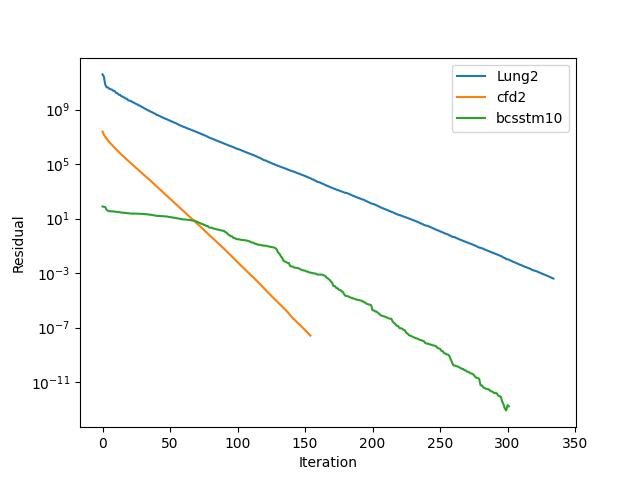
\includegraphics[width=\linewidth]{residuals_fast.jpg}
            \caption{}
            \label{fig:subfig1}
        \end{subfigure}
        \label{fig:fast}
    \end{minipage}%
    \begin{minipage}[b]{0.5\linewidth}
        \centering
        \begin{subfigure}{\linewidth}
            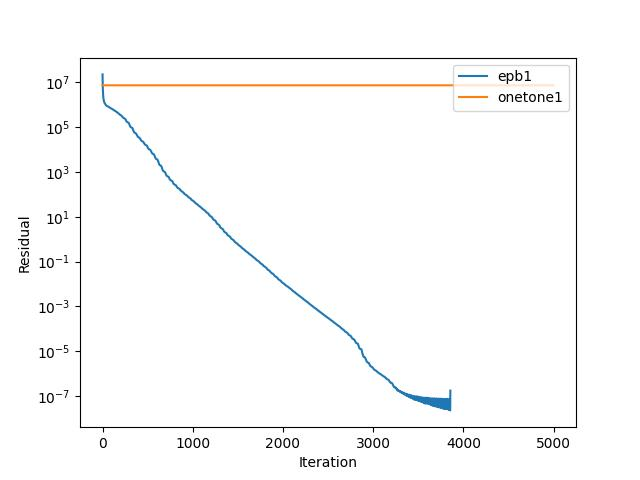
\includegraphics[width=\linewidth]{residuals_slow.jpg}
            \caption{}
            \label{fig:subfig2}
        \end{subfigure}
        \label{fig:slow}
    \end{minipage}
    \caption{Convergence plots of GMRES for the test matrices. (a) shows fast convergences and (b) slow or no convergence of GMRES}
    \label{fig:convergences}
\end{figure}
\subsubsection{Parallelization Performance}
\begin{table}[ht]
\centering
\begin{tabular}{|l|r|r|r|r|}
\hline
\rowcolor{gray!20}
\textbf{number of threads}     &  \textbf{1} &  \textbf{2}  &  \textbf{4}  &  \textbf{8}  \\
\hline
Lung2    & 2.52803     & 2.01759     & 1.63059     & 1.95627     \\
\hline
cfd2     & 1.50406     & 1.50657     & 1.09299     & 1.17903     \\
\hline
bcsstm10 & 0.098761    & 0.65573     & 0.725824    & 1.04566     \\
\hline
epb1     & 5.65513     & 8.87665     & 10.5441     & 14.9338     \\
\hline
onetone1  & 15.0989     & 18.0937     & 19.8476     & 25.4774     \\
\hline
\end{tabular}
\caption{Execution times for different processes.}

\label{tab:execution_times}
\end{table}

\begin{figure}[]
\centering
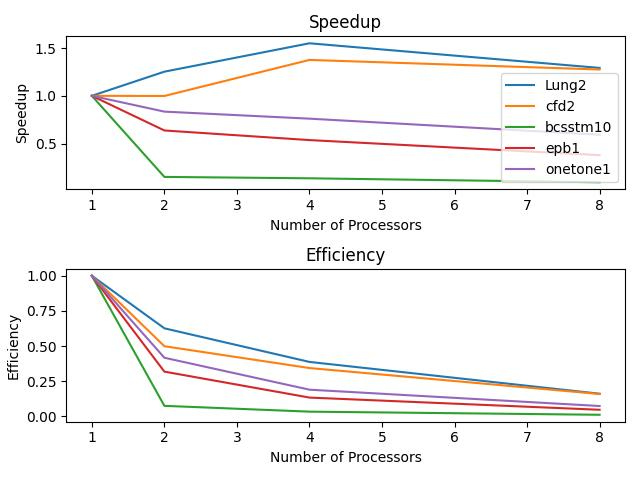
\includegraphics[width=0.7\linewidth]{metrics_testmats.jpg}
\caption{Speedup and Efficiency Metric for Test Matrices}

\label{fig:metrics-testmat}
\end{figure}


The runtimes for solving the linear system with the GMRES algorithm are shown in Table \ref{tab:execution_times} and some performance metrics are displayed in \ref{fig:metrics-testmat}.\\
For the SPD matrices \textit{lung} and \textit{cfd2} the runtime actually increases. This is the expected behaviour as the program has few steps where no parallelization can be applied and the datasize is very large (see Table \ref{tab:test-matrices}). The speedup is still bad as the optimal speedup is equal to the number of used processors. Additionally, the runtime increases when 8 threads are used. \\
The non SPD matrices on the other side increase their runtime with increasing number of threads. This behaviour is inexplicable as the data size is also big and the parallelization overhead neccessary to distribute the parallel processes on different threads should increase the runtime with such a large ratio. Additionally for comparable size the speedup is greater than 1 for the SPD matrices, but the influence on runtime should not depend on the property if SPD or not.
\newpage
\subsection{Solution of the Convection-Diffusion Equation}
Consider the  problem
$$
\frac{\partial}{\partial x}\left(D_{x} \frac{\partial c}{\partial x}\right)+\frac{\partial}{\partial y}\left(D_{y} \frac{\partial c}{\partial y}\right)-v_{x} \frac{\partial c}{\partial x}-v_{y} \frac{\partial c}{\partial y}=\frac{\partial c}{\partial t} \quad+f
$$
with the boundary conditions
$$
\begin{aligned}
	& c(x, t) = [x \in \Omega_1] \qquad & \text{for } x \in \Omega_1, t > 0 \\
	& c(x, t) = [x \in \Omega_2] \qquad & \text{for } x \in \Omega_2, t > 0 \\
\end{aligned}
$$
where the boundaries $\Omega_1$ and $\Omega_2$ are given by:
$$
\begin{aligned}
	& \Omega_1=\{(x, y):[x=0,0 \leq y \leq 1] \cup[0 \leq x \leq 0.3, y=0]\} \\
	& \Omega_2=\{(x, y):[x=1,0 \leq y \leq 1] \cup[0 \leq x \leq 1, y=1] \cup[0.3 \leq x \leq 1, y=0]\}
\end{aligned}
$$


The correct solution of this problem on the two different meshes is shown in \ref{fig:solution}. The solutions for small and big mesh should look the same but there occurred an error in the mesh creation for the big mesh and the boundary conditions are not created correctly. Because of the small size of the problem, it is not necessary to look at the performance for parallelization.\\
Unfortunately the evaluation for the big mesh could not be done because as mentioned the parallelization for the assembly which takes the most computational effort could not be resolved.

\begin{figure}[H]
	\begin{minipage}[b]{0.5\linewidth}
		\centering
		\begin{subfigure}{\linewidth}
			\centering
			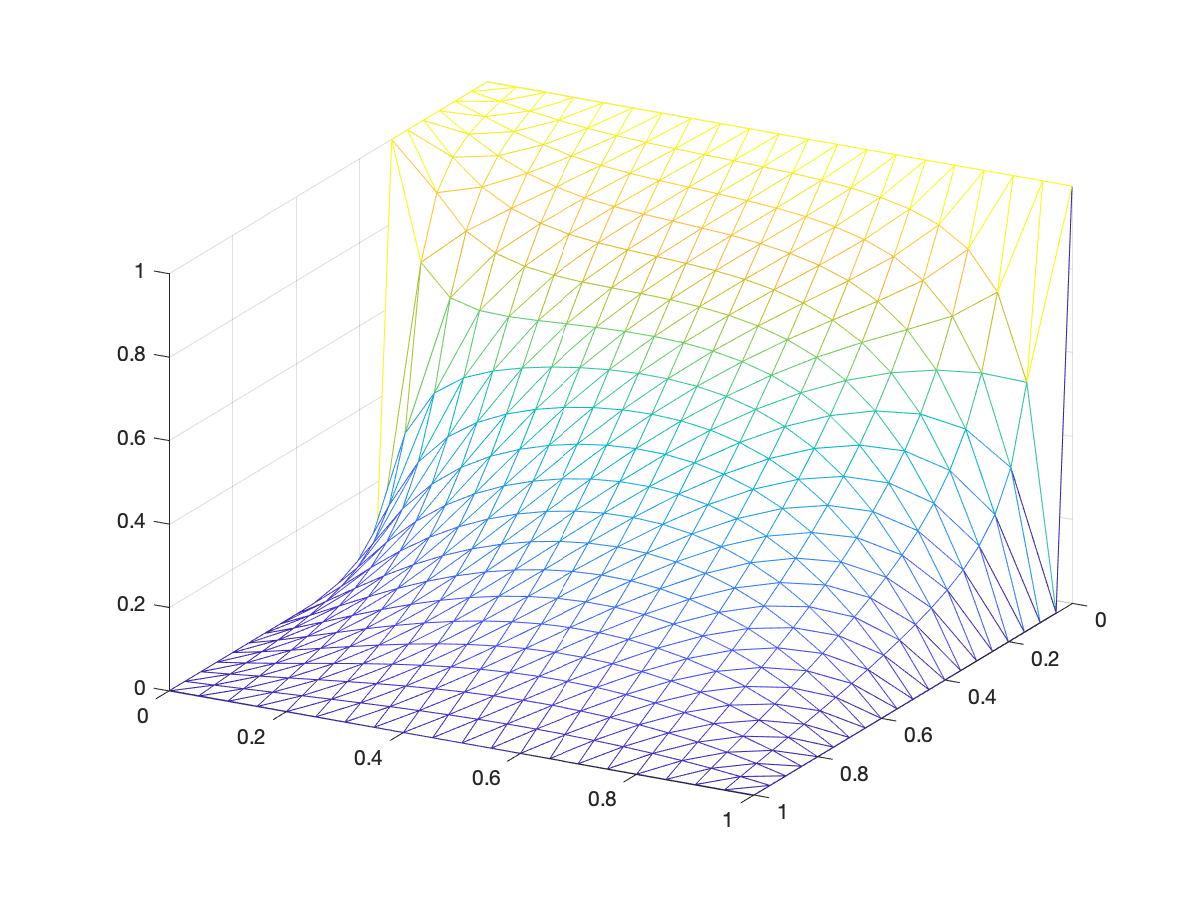
\includegraphics[width=0.7\linewidth]{small_solution_right}
			\caption{Solution for the small mesh}

		\end{subfigure}
			\label{fig:bigmeshnobound}
	\end{minipage}%
	\begin{minipage}[b]{0.5\linewidth}
		\centering
		\begin{subfigure}{\linewidth}
			\centering
			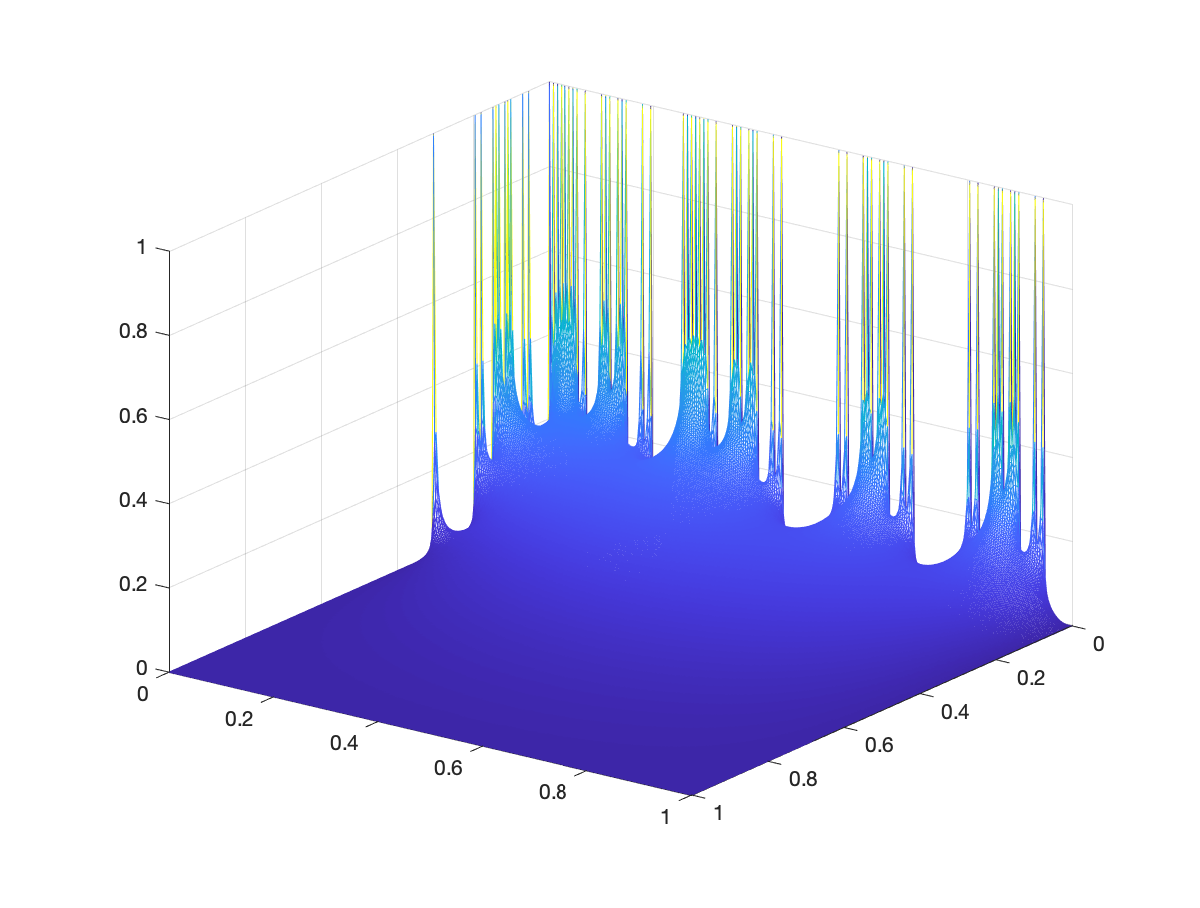
\includegraphics[width=0.7\linewidth]{bigmesh_nobound}

			\caption{Solution for the big mesh}
		\end{subfigure}
			\label{fig:smallsolutionright}
	\end{minipage}
	\caption{Solution of the Convection-Diffusion Problem.}
	\label{fig:solution}
\end{figure}



%\subsection{Performance of the Convection-Diffusion Problem}

\bibliographystyle{apalike}
\bibliography{sample}





\newpage

\begin{appendices}

\section{CPP Files}

\subsection{main.cpp}
\lstinputlisting[style=cppstyle]{main.cpp}
\label{code:main}


\subsection{GMRES.h}
\lstinputlisting[style=cppstyle]{GMRES.cpp}
\label{code:GMRES}


\subsection{functions.h}
\lstinputlisting[style=cppstyle]{functions.h}
\label{code:functions}

\subsection{fem\_functions.h}
\lstinputlisting[style=cppstyle]{fem_functions.h}
\label{code:femfunctions}


% Add more subsections for additional files if needed
\subsection{sparse.h}
\lstinputlisting[style=cppstyle]{sparse.h}
\label{code:sparse}

% Add more subsections for additional files if needed

\end{appendices}







\end{document}